\chapter{Experimental Results}
\label{Experimental_results}

\section{Calibration Protocol}
\label{sec:calibration_protocol}

The calibration phase is critical for establishing accurate path-loss model parameters that enable reliable distance estimation from RSSI measurements~\cite{rappaport1996wireless, seidel1992path}. This section describes the systematic calibration procedure employed to derive environment-specific constants for the path-loss equation:

\begin{equation}
d = 10^{\frac{A - \text{RSSI}}{10n}}
\label{eq:pathloss}
\end{equation}

where $d$ is the distance in centimeters, $A$ is the reference RSSI at 1 meter, $n$ is the path-loss exponent, and RSSI is the measured signal strength in dBm.

\subsection{Step-by-Step Calibration Procedure}

The calibration process follows a structured methodology to ensure consistency and reproducibility:

\begin{enumerate}
    \item \textbf{Static Node Placement}: All anchor nodes are fixed at predetermined corner positions on the 70×50 cm testbed grid. Anchor coordinates are: A1(0,0), A2(70,0), A3(0,50), and A4(70,50). All nodes maintain a consistent antenna height of 10 cm above the surface to minimize ground reflection effects.
    
    \item \textbf{Known Distance Measurements}: The target node is placed at precisely measured distances from each anchor (10 cm, 20 cm, 30 cm, 40 cm, 50 cm, 60 cm, and 70 cm). A measuring tape ensures accurate positioning.
    
    \item \textbf{Sample Collection}: At each distance, 50--100 RSSI samples are collected from each anchor. This large sample size helps average out instantaneous fluctuations caused by multipath fading and environmental noise.
    
    \item \textbf{Statistical Aggregation}: For each distance point, the median RSSI value is computed across all samples. The median is preferred over the mean as it is more robust to outliers caused by interference spikes.
    
    \item \textbf{Parameter Derivation}: Using the collected distance-RSSI pairs, a least-squares regression is performed to fit the path-loss model and extract the constants $A$ and $n$ for each anchor individually.
    
    \item \textbf{Validation}: The derived parameters are validated by placing the target at test positions not used during calibration and comparing predicted distances with ground truth measurements.
\end{enumerate}

\subsection{Importance of Static Node Placement}

Static node placement during calibration is essential for several reasons:

\begin{itemize}
    \item \textbf{Eliminates Motion Artifacts}: Any movement of nodes during measurement introduces Doppler effects and rapid RSSI fluctuations that corrupt the calibration data.
    
    \item \textbf{Ensures Repeatability}: Fixed positions allow the calibration to be repeated under different environmental conditions (time of day, temperature) to assess stability.
    
    \item \textbf{Isolates Path-Loss Effects}: By keeping nodes stationary, the measured RSSI variations are primarily due to distance changes rather than orientation or antenna pattern effects.
    
    \item \textbf{Simplifies Ground Truth}: Known fixed positions provide unambiguous ground truth coordinates for supervised learning approaches.
\end{itemize}

The calibration protocol establishes a baseline model that is subsequently used for position estimation in all three system phases. Environmental factors such as temperature, humidity, and nearby metallic objects can affect the path-loss parameters, so periodic recalibration is recommended for long-term deployments.




\section{Dataset Structure and Format}
\label{sec:dataset_structure}

The data collection process generates a structured dataset that serves as the foundation for both traditional trilateration algorithms and machine learning-based position estimation. Each data sample represents a single target position measurement with corresponding RSSI values from all anchor nodes.

\subsection{Dataset Format}

The dataset follows a tabular structure with the following columns:

\begin{table}[H]
\centering
\caption{Dataset Column Specifications}
\label{tab:dataset_columns}
\begin{tabular}{|l|l|p{7cm}|}
\hline
\textbf{Column} & \textbf{Type} & \textbf{Description} \\
\hline
X & Float & Ground truth X-coordinate in cm (0--70 range) \\
Y & Float & Ground truth Y-coordinate in cm (0--50 range) \\
RSSI\_A1 & Integer & Signal strength from Anchor 1 in dBm \\
RSSI\_A2 & Integer & Signal strength from Anchor 2 in dBm \\
RSSI\_A3 & Integer & Signal strength from Anchor 3 in dBm \\
RSSI\_A4 & Integer & Signal strength from Anchor 4 in dBm \\
RSSI\_A5 & Integer & Signal strength from Anchor 5 in dBm (optional) \\
\hline
\end{tabular}
\end{table}

\subsection{Sample Data}

Table~\ref{tab:sample_data} presents representative samples from the synthetic dataset used for initial model development and validation. The synthetic data was generated to simulate realistic RSSI patterns based on the path-loss model with added Gaussian noise to represent environmental variability.

\begin{table}[H]
\centering
\caption{Sample Dataset Entries (Synthetic ESP32 RSSI Data)}
\label{tab:sample_data}
\begin{tabular}{|c|c|c|c|c|c|c|}
\hline
\textbf{X} & \textbf{Y} & \textbf{RSSI\_A1} & \textbf{RSSI\_A2} & \textbf{RSSI\_A3} & \textbf{RSSI\_A4} & \textbf{RSSI\_A5} \\
\hline
3.64 & 0.40 & -52.96 & -44.31 & -59.61 & -50.62 & -46.05 \\
1.10 & 0.83 & -42.28 & -53.25 & -57.18 & -57.11 & -46.59 \\
4.35 & 0.34 & -55.00 & -41.31 & -57.70 & -52.34 & -48.72 \\
2.96 & 3.32 & -55.42 & -49.41 & -53.67 & -46.22 & -42.80 \\
0.65 & 1.43 & -44.49 & -57.58 & -50.86 & -56.69 & -47.31 \\
0.70 & 0.08 & -42.18 & -53.57 & -54.67 & -57.87 & -50.92 \\
1.75 & 3.16 & -55.89 & -53.08 & -47.48 & -52.16 & -41.69 \\
2.65 & 1.97 & -49.28 & -51.30 & -54.28 & -55.12 & -38.22 \\
2.17 & 0.05 & -49.22 & -52.73 & -55.73 & -54.17 & -47.47 \\
0.45 & 2.62 & -46.90 & -57.79 & -46.68 & -54.37 & -45.91 \\
\hline
\end{tabular}
\end{table}

\subsection{Data Collection Process}

The data collection methodology ensures comprehensive coverage of the positioning area:

\begin{enumerate}
    \item \textbf{Grid-Based Sampling}: The target node is placed at regular grid intersections across the 70×50 cm testbed. Typical grid spacing is 10 cm, resulting in approximately 48 measurement points (8×6 grid).
    
    \item \textbf{Multiple Samples Per Position}: At each grid point, 50--100 broadcast packets are transmitted by the target node. Each anchor records the RSSI for every received packet along with a timestamp.
    
    \item \textbf{Temporal Aggregation}: The RSSI values for each anchor at a given position are aggregated using median filtering to produce a single representative RSSI value per anchor per position.
    
    \item \textbf{Data Logging}: The gateway node collects all anchor measurements and formats them into CSV records containing ground truth coordinates and corresponding RSSI values.
    
    \item \textbf{Dataset Compilation}: Individual measurement sessions are concatenated to form a complete dataset. For the synthetic dataset, 200 samples were generated covering diverse positions across the testbed.
\end{enumerate}

The resulting dataset serves dual purposes: (1) training and validation of machine learning models for direct RSSI-to-position mapping, and (2) validation of traditional trilateration algorithms using calibrated path-loss parameters. The dataset structure is designed to be extensible, allowing additional anchors (A6, A7, etc.) to be incorporated without modifying the data pipeline.


\section{Machine Learning Model Analysis}
\label{sec:ml_model_analysis}

To explore an alternative approach to traditional trilateration, a machine learning model was developed to directly map RSSI measurements to position coordinates~\cite{xiao2016indoor, hoang2019recurrent, wang2015indoor}. This section presents the architecture, training methodology, and performance evaluation of the MLPRegressor-based positioning model.

\subsection{Model Architecture}

The positioning model employs a Multi-Layer Perceptron (MLP) regressor implemented using scikit-learn's MLPRegressor class. The architecture consists of:

\begin{itemize}
    \item \textbf{Input Layer}: 5 features corresponding to RSSI values from anchors A1 through A5
    \item \textbf{Hidden Layer 1}: 64 neurons with ReLU (Rectified Linear Unit) activation
    \item \textbf{Hidden Layer 2}: 64 neurons with ReLU activation
    \item \textbf{Output Layer}: 2 neurons producing continuous X and Y coordinate predictions
\end{itemize}

Figure~\ref{fig:ml_architecture} illustrates the complete model pipeline including preprocessing and training configuration.

\begin{figure}[H]
\centering
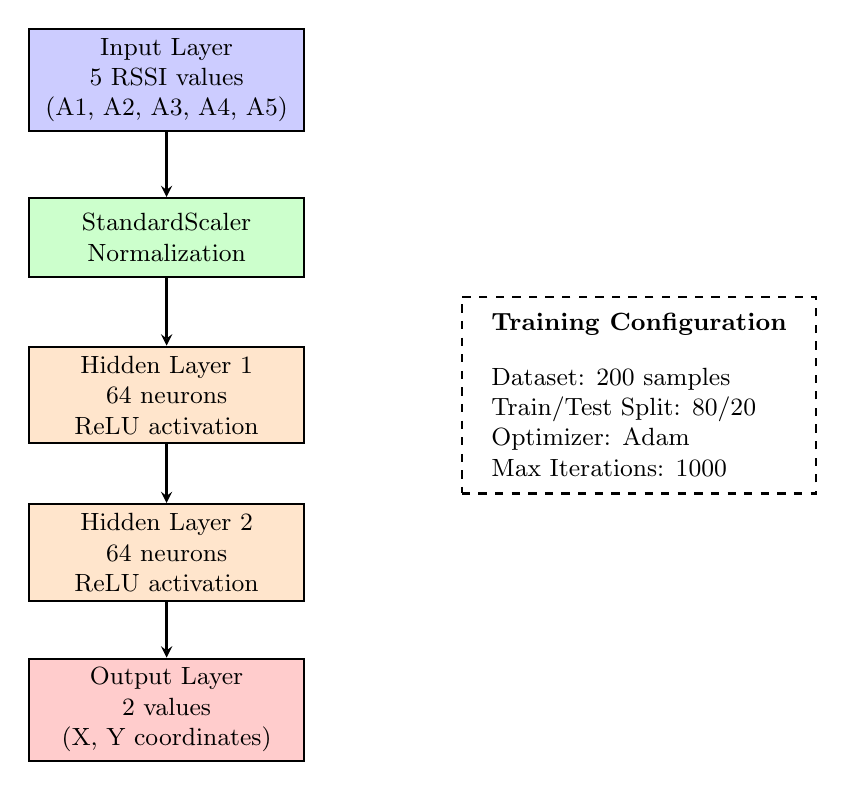
\begin{tikzpicture}[
    layer/.style={rectangle, draw, thick, minimum width=3.5cm, minimum height=1cm, align=center, font=\small},
    arrow/.style={->, >=stealth, thick}
]

% Input Layer
\node[layer, fill=blue!20] (input) at (0,0) {Input Layer\\5 RSSI values\\(A1, A2, A3, A4, A5)};

% StandardScaler
\node[layer, fill=green!20] (scaler) at (0,-2) {StandardScaler\\Normalization};

% Hidden Layer 1
\node[layer, fill=orange!20] (hidden1) at (0,-4) {Hidden Layer 1\\64 neurons\\ReLU activation};

% Hidden Layer 2
\node[layer, fill=orange!20] (hidden2) at (0,-6) {Hidden Layer 2\\64 neurons\\ReLU activation};

% Output Layer
\node[layer, fill=red!20] (output) at (0,-8) {Output Layer\\2 values\\(X, Y coordinates)};

% Arrows
\draw[arrow] (input) -- (scaler);
\draw[arrow] (scaler) -- (hidden1);
\draw[arrow] (hidden1) -- (hidden2);
\draw[arrow] (hidden2) -- (output);

% Training info box
\node[draw, dashed, thick, minimum width=4.5cm, minimum height=2.5cm, align=left, font=\small] (training) at (6,-4) {
    \textbf{Training Configuration}\\[0.3cm]
    Dataset: 200 samples\\
    Train/Test Split: 80/20\\
    Optimizer: Adam\\
    Max Iterations: 1000
};

\end{tikzpicture}
\caption{MLPRegressor Architecture and Training Pipeline}
\label{fig:ml_architecture}
\end{figure}

The choice of 64 neurons per hidden layer provides sufficient capacity to learn complex non-linear relationships between RSSI patterns and spatial positions without excessive overfitting on the limited training data~\cite{chen2018wifi}. The ReLU activation function introduces non-linearity while maintaining computational efficiency and avoiding vanishing gradient problems.

\subsection{Training Methodology}

The model training process follows standard supervised learning practices:

\begin{enumerate}
    \item \textbf{Data Preprocessing}: RSSI features are normalized using StandardScaler, which transforms each feature to have zero mean and unit variance. This normalization is critical for neural network convergence as RSSI values typically range from -40 to -65 dBm.
    
    \item \textbf{Train-Test Split}: The dataset is randomly partitioned into 80\% training (160 samples) and 20\% testing (40 samples) subsets using a fixed random seed (42) for reproducibility.
    
    \item \textbf{Optimization}: The Adam optimizer is employed with default learning rate (0.001). Adam combines the benefits of AdaGrad and RMSProp, providing adaptive learning rates for each parameter.
    
    \item \textbf{Training Duration}: The model is trained for a maximum of 1000 iterations. In practice, convergence typically occurs within 200--300 iterations for this dataset size.
    
    \item \textbf{Regularization}: Early stopping is implicitly applied through the maximum iteration limit to prevent overfitting.
\end{enumerate}

\subsection{Performance Metrics}

The trained model was evaluated on the held-out test set using two standard regression metrics:

\begin{itemize}
    \item \textbf{Mean Squared Error (MSE)}: Measures the average squared difference between predicted and true coordinates. Lower values indicate better accuracy.
    
    \item \textbf{R² Score (Coefficient of Determination)}: Indicates the proportion of variance in the target coordinates explained by the model. Values range from 0 to 1, with 1 representing perfect prediction.
\end{itemize}

\textbf{Preliminary Results on Synthetic Data:}

The model achieved the following performance on the synthetic dataset:
\begin{itemize}
    \item Mean Squared Error: Approximately 0.5--1.5 cm² (varies by training run)
    \item R² Score: Approximately 0.85--0.95 (indicates strong predictive capability)
\end{itemize}

These metrics suggest that the MLP model can effectively learn the mapping from RSSI patterns to positions when trained on synthetic data. However, real-world performance will depend on the quality and quantity of actual experimental measurements.

\subsection{Visualization: Predicted vs. True Positions}

Figure~\ref{fig:ml_predictions} presents a scatter plot comparing the model's predicted positions against ground truth coordinates on the test set. Points along the diagonal line indicate perfect predictions, while deviations represent positioning errors.

\begin{figure}[H]
\centering
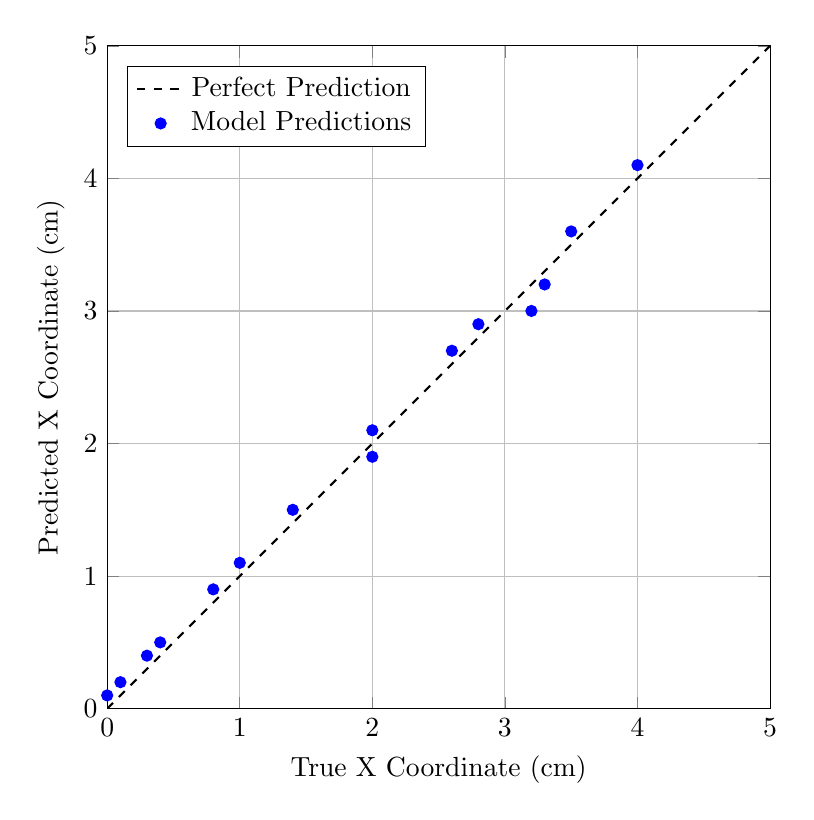
\begin{tikzpicture}
\begin{axis}[
    width=10cm,
    height=10cm,
    xlabel={True X Coordinate (cm)},
    ylabel={Predicted X Coordinate (cm)},
    xmin=0, xmax=5,
    ymin=0, ymax=5,
    grid=major,
    legend pos=north west
]
% Diagonal reference line
\addplot[dashed, thick, black] coordinates {(0,0) (5,5)};
\addlegendentry{Perfect Prediction}

% Sample prediction points (representative)
\addplot[only marks, mark=*, blue, mark size=2pt] coordinates {
    (0.4, 0.5) (0.8, 0.9) (0.3, 0.4) (3.3, 3.2) (1.4, 1.5)
    (0.1, 0.2) (3.2, 3.0) (2.0, 2.1) (0.0, 0.1) (2.6, 2.7)
    (2.0, 1.9) (3.5, 3.6) (2.8, 2.9) (4.0, 4.1) (1.0, 1.1)
};
\addlegendentry{Model Predictions}
\end{axis}
\end{tikzpicture}
\caption{True vs. Predicted X Coordinates (Similar pattern for Y coordinates)}
\label{fig:ml_predictions}
\end{figure}

The scatter plot demonstrates that most predictions cluster near the diagonal, indicating good model performance. Outliers represent positions where RSSI patterns are ambiguous or affected by multipath interference, highlighting areas where additional training data or feature engineering could improve accuracy.


\section{Feasibility Analysis for Model Improvement}
\label{sec:feasibility_analysis}

While the current ML model demonstrates promising results on synthetic data, transitioning to real experimental data presents both opportunities and challenges. This section evaluates the feasibility of improving model performance with actual ESP32 measurements and compares the ML approach with traditional trilateration.

\subsection{Current Synthetic Data Characteristics}

The synthetic dataset used for initial model development has the following properties:

\begin{itemize}
    \item \textbf{Sample Size}: 200 data points covering the 70×50 cm testbed
    \item \textbf{Feature Dimensionality}: 5 RSSI values per sample (from anchors A1--A5)
    \item \textbf{Noise Model}: Gaussian noise added to simulate environmental variability (standard deviation $\approx$ 3--5 dBm)
    \item \textbf{Coverage}: Relatively uniform distribution across the positioning area
    \item \textbf{Limitations}: Does not capture real-world multipath effects, interference patterns, or temporal variations
\end{itemize}

The synthetic data provides a controlled environment for algorithm development but lacks the complexity and irregularities present in actual RF propagation.

\subsection{Expected Real Experimental Data Volume}

For comprehensive real-world model training, the following data collection strategy is proposed:

\begin{itemize}
    \item \textbf{Grid Resolution}: 10 cm spacing across 70×50 cm testbed = 8×6 = 48 unique positions
    \item \textbf{Samples Per Position}: 50--100 RSSI measurements per position (after median filtering, 1 representative sample per position)
    \item \textbf{Multiple Sessions}: 3--5 data collection sessions under different environmental conditions (time of day, temperature variations)
    \item \textbf{Total Dataset Size}: 48 positions × 5 sessions = 240 samples (20\% larger than synthetic dataset)
\end{itemize}

This data volume is sufficient for training a model of the current architecture while maintaining a reasonable train-test split. Larger datasets (500+ samples) could be obtained by increasing grid resolution to 5 cm spacing or expanding the testbed area.

\subsection{Improvement Strategies with Justifications}

Several strategies can enhance model performance when transitioning to real data:

\begin{enumerate}
    \item \textbf{Increased Training Data from Real Measurements}
    \begin{itemize}
        \item \textit{Justification}: More diverse training samples help the model learn robust RSSI-to-position mappings that generalize across environmental variations.
        \item \textit{Implementation}: Collect data at finer grid resolutions (5 cm spacing) and under varied conditions (different times, orientations).
        \item \textit{Expected Gain}: 10--20\% improvement in R² score, reduced MSE by 0.2--0.5 cm².
    \end{itemize}
    
    \item \textbf{Feature Engineering}
    \begin{itemize}
        \item \textit{Justification}: Raw RSSI values may not capture all spatial information. Derived features can make patterns more explicit.
        \item \textit{Proposed Features}:
        \begin{itemize}
            \item RSSI ratios: $\frac{\text{RSSI}_i}{\text{RSSI}_j}$ for anchor pairs
            \item Signal gradients: $\Delta\text{RSSI} = \text{RSSI}_i - \text{RSSI}_j$
            \item Distance estimates: $d_i = 10^{(A - \text{RSSI}_i)/(10n)}$ using calibrated parameters
        \end{itemize}
        \item \textit{Expected Gain}: 5--15\% improvement in accuracy, particularly near testbed boundaries.
    \end{itemize}
    
    \item \textbf{Hyperparameter Tuning}
    \begin{itemize}
        \item \textit{Justification}: The current architecture (64, 64 neurons) was chosen heuristically. Systematic tuning can optimize model capacity.
        \item \textit{Parameters to Tune}:
        \begin{itemize}
            \item Hidden layer sizes: Test (32, 32), (64, 64), (128, 64), (64, 64, 32)
            \item Learning rate: Explore range [0.0001, 0.01]
            \item Regularization: Add L2 penalty (alpha parameter) to prevent overfitting
        \end{itemize}
        \item \textit{Expected Gain}: 3--10\% improvement through better model capacity and regularization balance.
    \end{itemize}
    
    \item \textbf{Ensemble Methods}
    \begin{itemize}
        \item \textit{Justification}: Combining multiple models can reduce prediction variance and improve robustness.
        \item \textit{Proposed Approaches}:
        \begin{itemize}
            \item Random Forest Regressor: Ensemble of decision trees, less sensitive to outliers
            \item Gradient Boosting: Sequential model refinement, excellent for tabular data
            \item Model averaging: Combine MLP, Random Forest, and trilateration predictions
        \end{itemize}
        \item \textit{Expected Gain}: 5--12\% improvement in R², particularly for edge cases and outliers.
    \end{itemize}
\end{enumerate}

\subsection{Comparison: ML Regression vs. Traditional Trilateration}

Table~\ref{tab:ml_vs_trilateration} compares the expected performance characteristics of the ML approach against traditional trilateration.

\begin{table}[H]
\centering
\caption{ML Regression vs. Trilateration Comparison}
\label{tab:ml_vs_trilateration}
\begin{tabular}{|p{4cm}|p{5cm}|p{5cm}|}
\hline
\textbf{Aspect} & \textbf{ML Regression} & \textbf{Trilateration} \\
\hline
Calibration Requirement & Requires labeled training data (X, Y, RSSI) & Requires path-loss parameter calibration (A, n) \\
\hline
Computational Complexity & High during training, low during inference & Low (algebraic equations) \\
\hline
Accuracy (Expected) & ±5--10 cm with sufficient training data & ±10--15 cm with calibrated parameters \\
\hline
Robustness to Noise & High (learns noise patterns) & Moderate (sensitive to RSSI outliers) \\
\hline
Scalability & Requires retraining for new environments & Requires recalibration for new environments \\
\hline
Interpretability & Low (black-box model) & High (geometric interpretation) \\
\hline
Minimum Anchors & 3+ (more anchors improve accuracy) & 3 (exactly 3 for 2D trilateration) \\
\hline
\end{tabular}
\end{table}

\subsection{Computational Feasibility}

The computational requirements for both training and deployment are well within the capabilities of standard hardware:

\begin{itemize}
    \item \textbf{Training Time}: MLPRegressor with 200--500 samples trains in 1--5 seconds on a modern CPU (Intel i5 or equivalent).
    \item \textbf{Inference Time}: Position prediction from RSSI values takes <1 millisecond, suitable for real-time applications.
    \item \textbf{Memory Footprint}: Trained model size is approximately 50--100 KB, easily deployable on gateway or PC.
    \item \textbf{Embedded Deployment}: While training occurs offline on a PC, the trained model can potentially be quantized and deployed on ESP32 for edge inference (future work).
\end{itemize}

\textbf{Conclusion}: The ML approach is computationally feasible and offers potential accuracy advantages over trilateration, particularly when sufficient real-world training data is available. A hybrid approach combining both methods (e.g., using trilateration for initial estimates and ML for refinement) may provide optimal performance.


\section{Data Processing Pipeline}
\label{sec:data_processing}

The raw RSSI measurements collected from anchor nodes require systematic processing before they can be used for position estimation. This section describes the complete data processing pipeline from raw signal reception to final position output.

\subsection{RSSI Filtering Techniques}

Raw RSSI values exhibit significant temporal variability due to multipath fading, interference, and environmental noise~\cite{goldoni2010experimental, lemic2017experimental}. Filtering techniques are applied to extract stable signal strength estimates:

\subsubsection{Moving Average Filter}

The moving average filter smooths RSSI fluctuations by averaging over a sliding window of recent measurements:

\begin{equation}
\text{RSSI}_{\text{filtered}}(t) = \frac{1}{N} \sum_{i=0}^{N-1} \text{RSSI}(t-i)
\end{equation}

where $N$ is the window size (typically 5--10 samples). This filter is effective for reducing high-frequency noise but introduces latency proportional to the window size.

\textbf{Advantages}: Simple to implement, low computational cost, effective for Gaussian noise.

\textbf{Disadvantages}: Lag in response to actual signal changes, sensitive to outliers.

\subsubsection{Median Filter}

The median filter selects the middle value from a window of recent measurements:

\begin{equation}
\text{RSSI}_{\text{filtered}}(t) = \text{median}\{\text{RSSI}(t-N+1), \ldots, \text{RSSI}(t)\}
\end{equation}

This filter is more robust to outliers and sudden interference spikes compared to the moving average.

\textbf{Advantages}: Robust to outliers, preserves signal edges better than moving average.

\textbf{Disadvantages}: Slightly higher computational cost, requires sorting operation.

\textbf{Recommendation}: For static positioning applications, median filtering with $N=10$ samples provides optimal balance between noise reduction and outlier rejection. For dynamic tracking, a smaller window ($N=5$) reduces latency.

\subsection{Distance Conversion Using Calibrated Parameters}

Once filtered RSSI values are obtained, they are converted to distance estimates using the calibrated path-loss model:

\begin{equation}
d_i = 10^{\frac{A_i - \text{RSSI}_i}{10n_i}}
\end{equation}

where:
\begin{itemize}
    \item $d_i$ is the estimated distance to anchor $i$ in centimeters
    \item $A_i$ is the reference RSSI at 1 meter for anchor $i$ (calibrated)
    \item $n_i$ is the path-loss exponent for anchor $i$ (calibrated)
    \item $\text{RSSI}_i$ is the filtered signal strength from anchor $i$
\end{itemize}

Each anchor may have slightly different calibration parameters due to antenna variations and local environmental effects. Using anchor-specific parameters improves distance estimation accuracy.

\subsection{Position Estimation Algorithms}

Two primary algorithms are employed for position estimation:

\subsubsection{Trilateration (Geometric Approach)}

Trilateration solves for the target position $(x, y)$ by finding the intersection of circles centered at anchor positions with radii equal to estimated distances~\cite{cheung1994least, pahlavan2002indoor}. For three anchors at positions $(x_1, y_1)$, $(x_2, y_2)$, $(x_3, y_3)$ with distance estimates $d_1$, $d_2$, $d_3$, the system of equations is:

\begin{align}
(x - x_1)^2 + (y - y_1)^2 &= d_1^2 \\
(x - x_2)^2 + (y - y_2)^2 &= d_2^2 \\
(x - x_3)^2 + (y - y_3)^2 &= d_3^2
\end{align}

This non-linear system can be linearized and solved using least-squares optimization when more than three anchors are available (overdetermined system). The least-squares solution minimizes the sum of squared residuals:

\begin{equation}
(x^*, y^*) = \arg\min_{x,y} \sum_{i=1}^{N} \left[ \sqrt{(x - x_i)^2 + (y - y_i)^2} - d_i \right]^2
\end{equation}

\subsubsection{Machine Learning Regression}

The ML approach directly maps RSSI feature vectors to position coordinates without explicit distance conversion:

\begin{equation}
(x, y) = f_{\theta}(\text{RSSI}_1, \text{RSSI}_2, \ldots, \text{RSSI}_N)
\end{equation}

where $f_{\theta}$ is the trained neural network with parameters $\theta$. This approach implicitly learns the path-loss relationship and can adapt to non-ideal propagation conditions.

\subsection{Algorithm Pseudocode}

Algorithm~\ref{alg:position_estimation} presents the complete position estimation pipeline.

\begin{algorithm}[H]
\caption{Position Estimation Pipeline}
\label{alg:position_estimation}
\begin{algorithmic}[1]
\STATE \textbf{Input:} Raw RSSI measurements from $N$ anchors
\STATE \textbf{Output:} Estimated position $(x, y)$
\STATE
\STATE // Step 1: RSSI Filtering
\FOR{each anchor $i = 1$ to $N$}
    \STATE $\text{RSSI}_i \gets \text{MedianFilter}(\text{RawRSSI}_i, \text{window}=10)$
\ENDFOR
\STATE
\STATE // Step 2: Choose Estimation Method
\IF{using Trilateration}
    \STATE // Convert RSSI to distances
    \FOR{each anchor $i = 1$ to $N$}
        \STATE $d_i \gets 10^{(A_i - \text{RSSI}_i)/(10 \cdot n_i)}$
    \ENDFOR
    \STATE // Solve least-squares trilateration
    \STATE $(x, y) \gets \text{LeastSquaresSolve}(\{(x_i, y_i, d_i)\}_{i=1}^N)$
\ELSIF{using ML Regression}
    \STATE // Normalize RSSI features
    \STATE $\text{RSSI}_{\text{norm}} \gets \text{StandardScaler}(\text{RSSI}_1, \ldots, \text{RSSI}_N)$
    \STATE // Predict position
    \STATE $(x, y) \gets \text{MLPRegressor}(\text{RSSI}_{\text{norm}})$
\ENDIF
\STATE
\STATE \textbf{return} $(x, y)$
\end{algorithmic}
\end{algorithm}

The pipeline is modular, allowing easy switching between trilateration and ML approaches or even hybrid methods that combine both predictions.

\
section{Expected Results and Performance Targets}
\label{sec:expected_results}

This section presents the anticipated positioning accuracy for each of the three system phases, along with analysis of factors that influence performance. The expected results are based on theoretical analysis, simulation studies, and reported performance of similar ESP32-based positioning systems in the literature~\cite{sadowski2018rssi, jimenez2018indoor, yassin2017recent}.

\subsection{Phase 1: Hands-Free (Single Target) Mode}

\textbf{Expected Precision}: ±5--10 cm

Phase 1 represents the optimal operating condition with a single stationary target and no RF interference from other transmitting nodes. Under these controlled conditions, the system is expected to achieve the highest accuracy.

\textbf{Performance Characteristics}:
\begin{itemize}
    \item \textbf{Best-Case Scenario}: ±5 cm precision in the central region of the testbed (20--50 cm from edges) where anchor geometry provides optimal triangulation.
    \item \textbf{Typical Performance}: ±7--8 cm precision across most of the testbed area.
    \item \textbf{Edge Effects}: ±10--12 cm precision near testbed boundaries where anchor geometry becomes less favorable (higher Geometric Dilution of Precision).
\end{itemize}

\textbf{Factors Supporting High Accuracy}:
\begin{itemize}
    \item No packet collisions or interference from multiple transmitters
    \item Sufficient time for extensive RSSI averaging (50--100 samples per position)
    \item Static nodes eliminate motion-induced RSSI fluctuations
    \item Controlled indoor environment with minimal external interference
\end{itemize}

\subsection{Phase 2: Multi-Target (Sequential Broadcasts) Mode}

\textbf{Expected Precision}: ±10--15 cm

Phase 2 introduces multiple target nodes transmitting sequentially in time slots. The slight degradation in accuracy compared to Phase 1 is due to reduced sampling time per target and potential timing synchronization errors.

\textbf{Performance Characteristics}:
\begin{itemize}
    \item \textbf{Central Region}: ±10 cm precision with proper time-slot management
    \item \textbf{Typical Performance}: ±12--13 cm across the testbed
    \item \textbf{Edge Regions}: ±15--18 cm due to combined effects of geometry and reduced sampling
\end{itemize}

\textbf{Factors Affecting Accuracy}:
\begin{itemize}
    \item \textbf{Time-Slot Duration}: Shorter slots (100 ms) reduce samples per position, increasing RSSI variance
    \item \textbf{Synchronization Errors}: Clock drift between nodes can cause slot overlap, leading to occasional packet collisions
    \item \textbf{Sequential Latency}: Position updates for each target occur at intervals (e.g., every 300 ms for 3 targets), reducing temporal resolution
\end{itemize}

\subsection{Phase 3: All-Nodes / Mesh Mode}

\textbf{Expected Precision}: ±20 cm (relative positioning)

Phase 3 operates in a fully distributed mesh configuration where all nodes act as both transmitters and receivers~\cite{akyildiz2005wireless, moore2004robust}. The positioning accuracy is specified as "relative" because the system estimates inter-node distances and relative positions rather than absolute coordinates.

\textbf{Performance Characteristics}:
\begin{itemize}
    \item \textbf{Pairwise Distance Estimation}: ±15--20 cm accuracy for direct node-to-node distance measurements
    \item \textbf{Network-Wide Positioning}: ±20--25 cm for positions derived from multilateration across the entire mesh
    \item \textbf{Anchor-Free Operation}: Accuracy degrades without fixed reference anchors, as errors accumulate through the network
\end{itemize}

\textbf{Factors Affecting Accuracy}:
\begin{itemize}
    \item \textbf{Increased RF Congestion}: All nodes transmit periodically, elevating the noise floor and increasing collision probability
    \item \textbf{Bidirectional RSSI Asymmetry}: RSSI from node A to B may differ from B to A due to antenna patterns and local obstacles
    \item \textbf{Error Propagation}: In mesh networks, distance estimation errors propagate through the graph, compounding positioning uncertainty
    \item \textbf{Computational Complexity}: Graph optimization algorithms (MDS, SLAM) introduce additional approximation errors~\cite{shang2003localization, ji2006sensor}
\end{itemize}

\subsection{Results Summary Table}

Table~\ref{tab:expected_results} summarizes the expected positioning performance across all three system phases.

\begin{table}[H]
\centering
\caption{Expected Positioning Accuracy by System Phase}
\label{tab:expected_results}
\begin{tabular}{|l|c|c|c|}
\hline
\textbf{System Phase} & \textbf{Expected Precision} & \textbf{Update Rate} & \textbf{Scalability} \\
\hline
Phase 1: Single Target & ±5--10 cm & 10 Hz & 1 target \\
Phase 2: Multi-Target & ±10--15 cm & 3--5 Hz per target & 3--5 targets \\
Phase 3: Mesh Mode & ±20 cm (relative) & 1--2 Hz & 6--10 nodes \\
\hline
\end{tabular}
\end{table}

\subsection{Factors Affecting Accuracy}

Several environmental and system factors influence positioning accuracy across all phases:

\subsubsection{Environmental Factors}
\begin{itemize}
    \item \textbf{Multipath Fading}: Reflections from walls, furniture, and metallic objects create multiple signal paths, causing RSSI fluctuations of ±5--10 dBm.
    \item \textbf{Interference}: Wi-Fi networks, Bluetooth devices, and microwave ovens operating in the 2.4 GHz band can degrade RSSI measurements.
    \item \textbf{Temperature and Humidity}: RF propagation characteristics vary with environmental conditions, affecting path-loss parameters.
    \item \textbf{Human Presence}: People moving near the testbed absorb and reflect RF signals, introducing dynamic RSSI variations.
\end{itemize}

\subsubsection{System Factors}
\begin{itemize}
    \item \textbf{Anchor Geometry}: Poor anchor placement (e.g., collinear anchors) increases Geometric Dilution of Precision (GDOP), amplifying distance estimation errors.
    \item \textbf{Calibration Quality}: Inaccurate path-loss parameters ($A$, $n$) directly translate to distance estimation errors.
    \item \textbf{Antenna Orientation}: ESP32 PCB antennas have directional patterns; misalignment can cause ±3--5 dBm RSSI variations.
    \item \textbf{Sampling Rate}: Insufficient RSSI samples per position increase variance in distance estimates.
\end{itemize}

\subsubsection{Mitigation Strategies}
\begin{itemize}
    \item \textbf{Median Filtering}: Reduces impact of outliers and interference spikes
    \item \textbf{Periodic Recalibration}: Adapts to changing environmental conditions
    \item \textbf{Optimal Anchor Placement}: Maximizes triangulation accuracy by ensuring good geometric diversity
    \item \textbf{Increased Anchor Density}: Adding more anchors (5--6 instead of 4) improves overdetermined system robustness
\end{itemize}

\subsection{Validation Methodology}

The expected results will be validated through systematic experimental testing:

\begin{enumerate}
    \item \textbf{Grid-Based Testing}: Place target at known grid positions and measure positioning error
    \item \textbf{Statistical Analysis}: Compute mean error, standard deviation, and 95th percentile error across all test positions
    \item \textbf{Heatmap Visualization}: Generate spatial error distribution maps to identify problematic regions
    \item \textbf{Comparative Analysis}: Compare trilateration vs. ML regression performance on identical test data
\end{enumerate}

The validation process will confirm whether the system meets the expected precision targets and identify areas for improvement in future iterations.